\documentclass[
	classe=1 STI2D,
	gray,
	surFeuille,
	headerTitle=Évaluation\space Chapitre\space 2
]{évaluation}

\usepackage{tcolorbox}
\usepackage{tkz-tab}
\usetikzlibrary{calc}

\title{[CORRECTION] Évaluation : Généralités sur les fonctions (sujet A)}
\author{}
\date{}

\begin{document}

\maketitle

\begin{exercice}
	\begin{enumerate}
		\item L'image par $f$ de $-4$ est $-2$.

		      L'image par $f$ de $0$ est $-3$
		\item Sur $[1 ; 5]$, $f$ est croissante.
		\item Le taux de variation de $f$ entre $-2$ et $2$ est
		      \begin{align*}
			      \frac{f(2) - f(-2)}{2 - (-2)} & = \frac{-1 - 3}{2 + 2} \\
			                                    & = \frac{-4}{4}         \\
			                                    & = -1
		      \end{align*}
		\item L'image par $g$ de $-2$ est $1$

		      L'image par $g$ de $5$ est $4$
		\item Les antécédents par $g$ de $-1$ sont $-4$ et $2$.

		      Les antécédents par $g$ de $1$ sont $-2$ et $4$.

		      $5$ n'a pas d'antécédents par $g$.
		\item 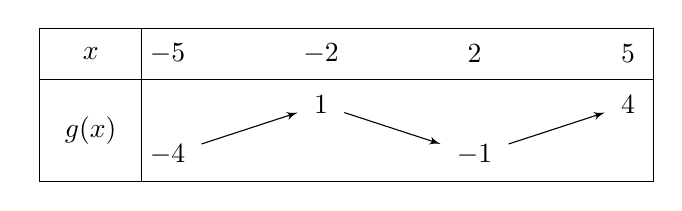
\begin{tikzpicture}[scale=0.65]
			      \tkzTabInit{$x$ / 1 , $g(x)$ / 2}{$-5$, $-2$, $2$, $5$}
			      \tkzTabVar{-/ $-4$, +/ $1$, -/ $-1$, +/ $4$}
		      \end{tikzpicture}
	\end{enumerate}
\end{exercice}

\begin{exercice}
	\begin{enumerate}
		\item \begin{align*}
			      f(x) = 0 & ⇔ 3x + 2 = 0         \\
			               & ⇔  3x = -2           \\
			               & ⇔   x = -\frac{2}{3}
		      \end{align*}
		\item 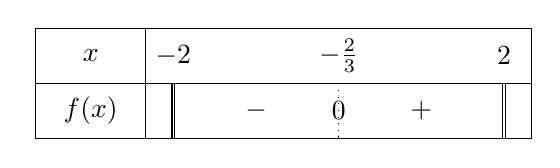
\begin{tikzpicture}[scale=0.7]
			      \tkzTabInit{$x$ / 1 , $f(x)$ / 1}{$-2$, $-\frac{2}{3}$, $2$}
			      \tkzTabLine{d, -, z, +, d}
		      \end{tikzpicture}
		\item Le taux de variation de $f$ entre $-2$ et $2$ est :
		      \begin{align*}
			      \frac{f(2) - f(-2)}{2 - (-2)} & = \frac{(3×2 + 2) - (3×(-2) + 2)}{2 + 2} \\
			                                    & = \frac{8 - (-4)}{4}                     \\
			                                    & = \frac{12}{4}                           \\
			                                    & = 3
		      \end{align*}
		\item Le taux de variation de $f$ entre $3$ et $6$ est
		      \begin{align*}
			      \frac{f(6) - f(3)}{6 - 3} & = \frac{(3×6 + 2) - (3×3 + 2)}{3} \\
			                                & = \frac{20 - 11}{3}               \\
			                                & = \frac{9}{3}                     \\
			                                & = 3
		      \end{align*}
		\item Soient $a$ et $b$ deux nombres réels. Le taux de variation de $f$ entre $a$ et $b$ est alors
		      \begin{align*}
			      \frac{f(b) - f(a)}{b - a} & = \frac{(3×b + 2) - (3×a + 2)}{b - a} \\
			                                & = \frac{3×(b - a) + 2 - 2}{b - a}     \\
			                                & = \frac{3×(b - a)}{b - a}             \\
			                                & = 3
		      \end{align*}
	\end{enumerate}
\end{exercice}

\begin{exercice}
	\begin{enumerate}
		\item On appelle $x$ le nombre de mois écoulés.

		      Avec la stratégie d'origine, l'entreprise dépense $6\ 250€$ par mois : le coût au bout de $x$ mois est donc $6\ 250 × x$.

		      Avec la nouvelle stratégie, l'entreprise dépense $120\ 000€$ initialement, puis $2\ 500 + \frac{9\ 600}{12} = 3\ 300€$ par mois. Le coût au bout de $x$ mois est donc $120\ 000 + 3\ 300 × x$.

		      On cherche  donc $x$ tel que
		      \begin{align*}
			      6\ 250x & > 120\ 000 + 3\ 300x \\
			      2\ 950x & > 120\ 000           \\
			      x       & > 40,67...
		      \end{align*}

		      Il faut donc attendre au moins $41$ mois avant que la nouvelle méthode soit meilleure.
		\item L'entreprise gagne à présent $250 × 5 = 1\ 250€$ par mois. Le coût au bout de $x$ mois est donc à présent $120\ 000 + 3\ 300x - 1\ 250x = 120\ 000 + 2\ 050x$.

		      On cherche donc $x$ tel que
		      \begin{align*}
			      6\ 250x & > 120\ 000 + 2\ 050x \\
			      4\ 200x & > 120\ 000           \\
			      x       & > 28,57...
		      \end{align*}

		      Il faut donc attendre au moins $29$ mois avant que la nouvelle méthode soit meilleure.
	\end{enumerate}
\end{exercice}

\begin{exercice}
	\begin{enumerate}
		\item $𝒜₁(x) = x × (x+1) = x² + x$ cm²
		\item $𝒜₂(x) = \frac{6×x}{2} + \frac{4×x}{2} = 5x$ cm²
		\item \begin{tikzpicture}
			      \draw[->] (0,0) -- (11,0) node[below] {$x$ (en cm)};
			      \draw[->] (0,0) -- (0,13) node[left] {aire (en cm²)};
			      \foreach \x in {0,...,10} {
					      \draw (\x,0) -- ++(0,-0.2) node[below] {$\x$};
				      }
			      \foreach \y in {1,...,12} {
					      \draw (0, \y) -- ++(-0.2,0) node[left] {$\y 0$};
				      }

			      \draw[blue,ultra thick,domain=0:10,variable=\x] plot({\x},{(\x*\x + \x)/10}) node[above] {$𝒜₁$};
			      \draw[red,ultra thick,domain=0:10,variable=\x] plot({\x},{(5*\x)/10}) node[above] {$𝒜₂$};
		      \end{tikzpicture}
		\item Les deux aires sont égales lorsque $x = 4$ cm. L'aire est alors de $20$ cm².
	\end{enumerate}
\end{exercice}

\end{document}